\documentclass[a4paper,10pt]{article}

\usepackage[usenames,dvipsnames]{xcolor}
\usepackage[utf8]{inputenc}
\usepackage{tikz}
\usetikzlibrary{arrows,decorations.pathmorphing,backgrounds,positioning,fit,petri}
\renewcommand*{\familydefault}{\sfdefault}



\begin{document}

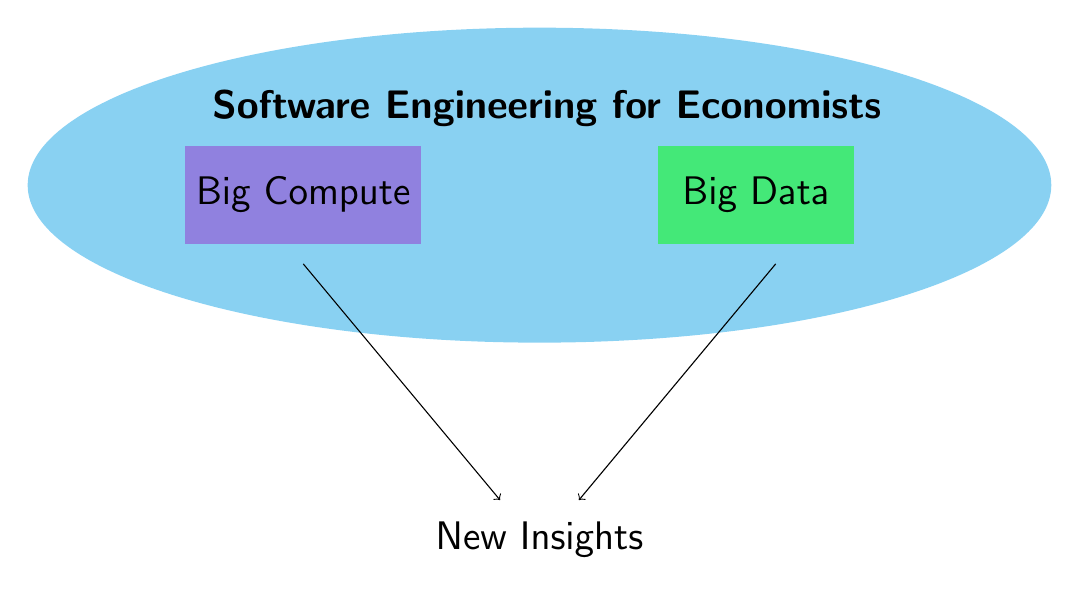
\begin{tikzpicture}
\fill[fill opacity=.5, text opacity=1, color=Cerulean] (0,0) ellipse (6.5 and 2) node[color = black,label={[yshift=0.5cm, color = black] \Large\textbf{ Software Engineering for Economists}}] {};  
\fill[fill opacity=.5, text opacity=1, color=green] (1.5,-0.75) rectangle (4.0,0.5) node[pos=.5, color = black] {\Large Big Data};
\fill[fill opacity=.5, text opacity=1, color=DarkOrchid] (-4.5,-0.75) rectangle (-1.5,0.5) node[pos=.5, color = black] {\Large Big Compute};
\path (-4, -5) rectangle (4.0,-4.0) node[pos=.5, color = black] {\Large{New Insights}};

% Connectors
\draw [->] (-3,-1) -- (-0.5,-4);
\draw [->] ( 3,-1) -- (0.5,-4);
\end{tikzpicture}


\end{document}
